\part*{Appendix}
\addcontentsline{toc}{chapter}{Appendix}
\renewcommand{\thesection}{\arabic{section}}
\renewcommand{\theequation}{\arabic{equation}}

\section{Visualized Effect of the Course \acl{seba} on the \acl{ei}}
\label{app:graphs}


\begin{figure}[H]
\centering
\begin{minipage}{.5\textwidth}
  \centering
  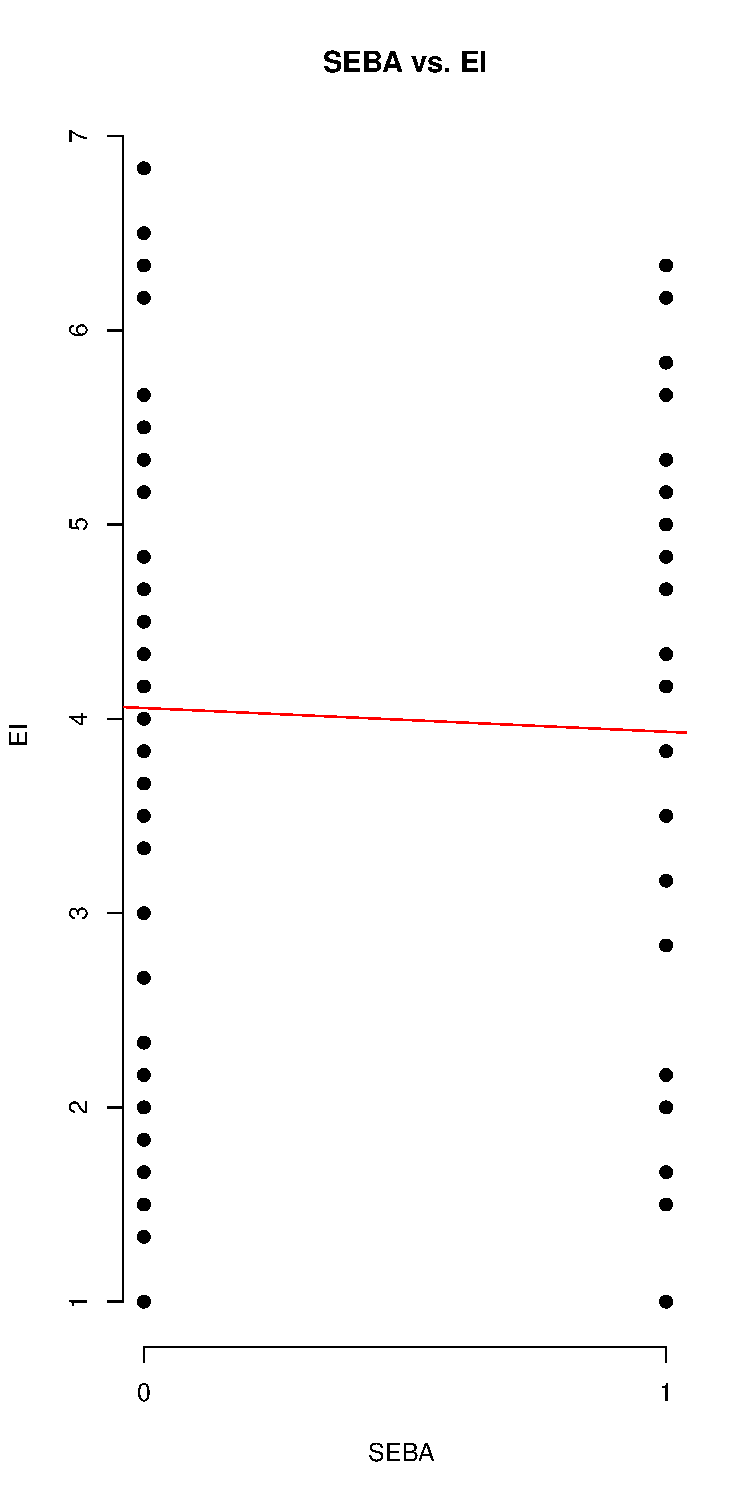
\includegraphics[width=.5\linewidth]{images/SEBAvsEI.pdf}
  \captionof{figure}{Scatterplot \ac{ei} $\sim $ \ac{seba}}
  \label{fig:test1}
\end{minipage}%
\begin{minipage}{.5\textwidth}
  \centering
  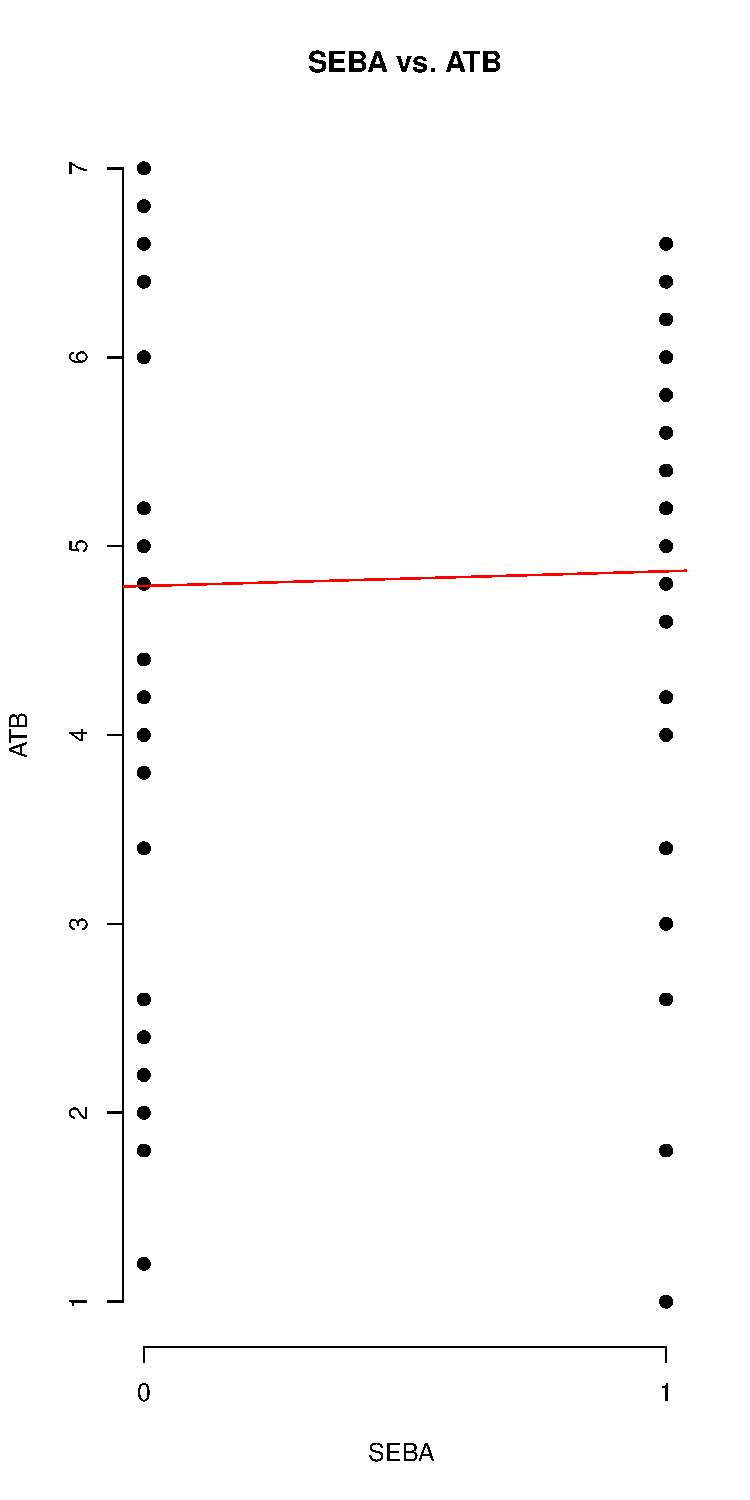
\includegraphics[width=.5\linewidth]{images/SEBAvsATB.pdf}
  \captionof{figure}{Scatterplot \ac{atb} $\sim $ \ac{seba}}
  \label{fig:test2}
\end{minipage}
\end{figure}

\begin{figure}[H]
\centering
\begin{minipage}{.5\textwidth}
  \centering  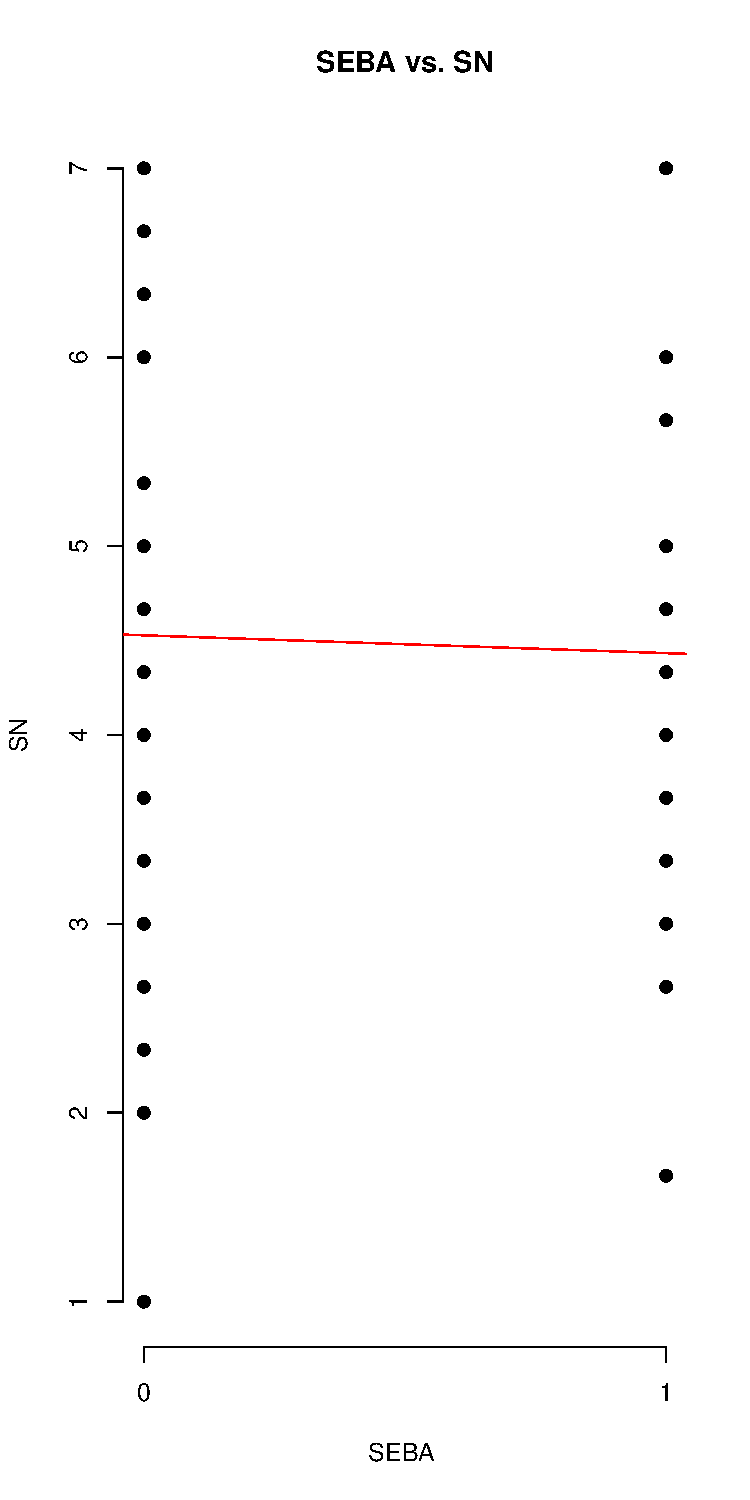
\includegraphics[width=.5\linewidth]{images/SEBAvsSN.pdf}
  \captionof{figure}{Scatterplot \ac{sn} $\sim $ \ac{seba}}
  \label{fig:test1}
\end{minipage}%
\begin{minipage}{.5\textwidth}
  \centering
  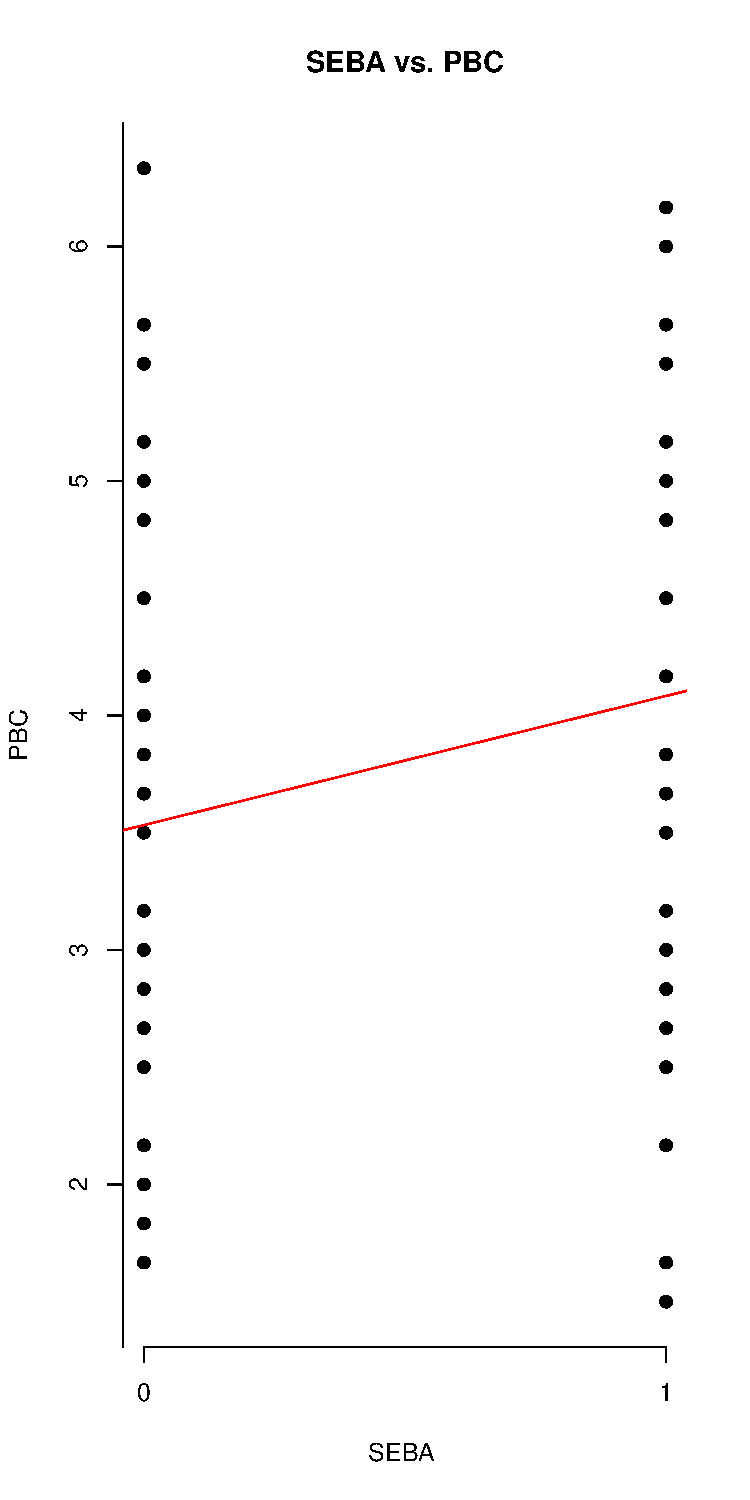
\includegraphics[width=.5\linewidth]{images/SEBAvsPBC.pdf}
  \captionof{figure}{Scatterplot \ac{pbc} $\sim $ \ac{seba}}
  \label{fig:test2}
\end{minipage}
\end{figure}

\clearpage

\section{Questionnaire}\label{app:questionaire}

This questionnaire is fully adapted from Li{\~n}{\'a}n and Chen 2009 \cite{linan2009development}.
\\

\large{Personal Attitude}
\\
\emph{11. Indicate your level of agreement with the following sentences from 1 (total disagreement) to 7 (total agreement).}

\begin{table}[H]
\scriptsize	
\centering

\begin{tabular}{p{10cm}lllllll}
\toprule
                                                                             & 1         & 2         & 3         & 4         & 5         & 6         & 7         \\ \midrule
11.a- Being an entrepreneur implies more advantages than disadvantages to me & $\square$ & $\square$ & $\square$ & $\square$ & $\square$ & $\square$ & $\square$ \\
11.b- A career as entrepreneur is attractive for me                          & $\square$ & $\square$ & $\square$ & $\square$ & $\square$ & $\square$ & $\square$ \\
11.c- If I had the opportunity and resources, I'd like to start a firm       & $\square$ & $\square$ & $\square$ & $\square$ & $\square$ & $\square$ & $\square$ \\
11.d- Being an entrepreneur would entail great satisfactions for me          & $\square$ & $\square$ & $\square$ & $\square$ & $\square$ & $\square$ & $\square$ \\
11.e- Among various options, I would rather be an entrepreneur               & $\square$ & $\square$ & $\square$ & $\square$ & $\square$ & $\square$ & $\square$ \\ \bottomrule
\end{tabular}
\end{table}

\large{Subjective Norm}
\\
\emph{13. If you decided to create a firm, would people in your close environment approve of that decision? Indicate from 1 (total disapproval) to 7 (total approval).}

\begin{table}[H]
\scriptsize	
\centering

\begin{tabular}{p{10cm}lllllll}
\toprule
                                                                             & 1         & 2         & 3         & 4         & 5         & 6         & 7         \\ \midrule
13.a-Your close family & $\square$ & $\square$ & $\square$ & $\square$ & $\square$ & $\square$ & $\square$ \\
13.b- Your friends                          & $\square$ & $\square$ & $\square$ & $\square$ & $\square$ & $\square$ & $\square$ \\
13.c- Your colleagues      & $\square$ & $\square$ & $\square$ & $\square$ & $\square$ & $\square$ & $\square$ \\ \bottomrule
\end{tabular}
\end{table}


\large{Perceived Behavioral Control}
\\
\emph{15. To what extent do you agree with the following statements regarding your entrepre- neurial capacity? Value them from 1 (total disagreement) to 7 (total agreement).}

\begin{table}[H]
\scriptsize	
\centering

\begin{tabular}{p{10cm}lllllll}
\toprule
                                                                               & 1         & 2         & 3         & 4         & 5         & 6         & 7         \\ \midrule
15.a- To start a firm and keep it working would be easy for me                  & $\square$ & $\square$ & $\square$ & $\square$ & $\square$ & $\square$ & $\square$ \\
15.b- I am prepared to start a viable firm                                      & $\square$ & $\square$ & $\square$ & $\square$ & $\square$ & $\square$ & $\square$ \\
15.c- I can control the creation process of a new firm                          & $\square$ & $\square$ & $\square$ & $\square$ & $\square$ & $\square$ & $\square$ \\
15.d- I know the necessary practical details to start a firm                    & $\square$ & $\square$ & $\square$ & $\square$ & $\square$ & $\square$ & $\square$ \\
15.e- I know how to develop an entrepreneurial project                          & $\square$ & $\square$ & $\square$ & $\square$ & $\square$ & $\square$ & $\square$ \\
15.f- If I tried to start a firm, I would have a high probability of succeeding & $\square$ & $\square$ & $\square$ & $\square$ & $\square$ & $\square$ & $\square$ \\ \bottomrule
\end{tabular}
\end{table}


\large{Entrepreneurial Intention}
\\
\emph{18. Indicate your level of agreement with the following statements from 1 (total disagree- ment) to 7 (total agreement).}

\begin{table}[H]
\scriptsize	
\centering

\begin{tabular}{p{10cm}lllllll}
\toprule
                                                                                                                                     & 1         & 2         & 3         & 4         & 5         & 6         & 7         \\ \midrule
18.a- I am ready to do anything to be an entrepreneur       & $\square$ & $\square$ & $\square$ & $\square$ & $\square$ & $\square$ & $\square$ \\
18.b- My professional goal is to become an entrepreneur     & $\square$ & $\square$ & $\square$ & $\square$ & $\square$ & $\square$ & $\square$ \\
18.c- I will make every effort to start and run my own firm & $\square$ & $\square$ & $\square$ & $\square$ & $\square$ & $\square$ & $\square$ \\
18.d- I am determined to create a firm in the future        & $\square$ & $\square$ & $\square$ & $\square$ & $\square$ & $\square$ & $\square$ \\
18.e- I have very seriously thought of starting a firm      & $\square$ & $\square$ & $\square$ & $\square$ & $\square$ & $\square$ & $\square$ \\ 
18.f- I have the firm intention to start a firm some day    & $\square$ & $\square$ & $\square$ & $\square$ & $\square$ & $\square$ & $\square$ \\ \bottomrule

\end{tabular}
\end{table}

\section{Survey Responses}\label{app:raw-data}
\begin{figure}[H]
\centering{
\caption{Raw Survey Responses}
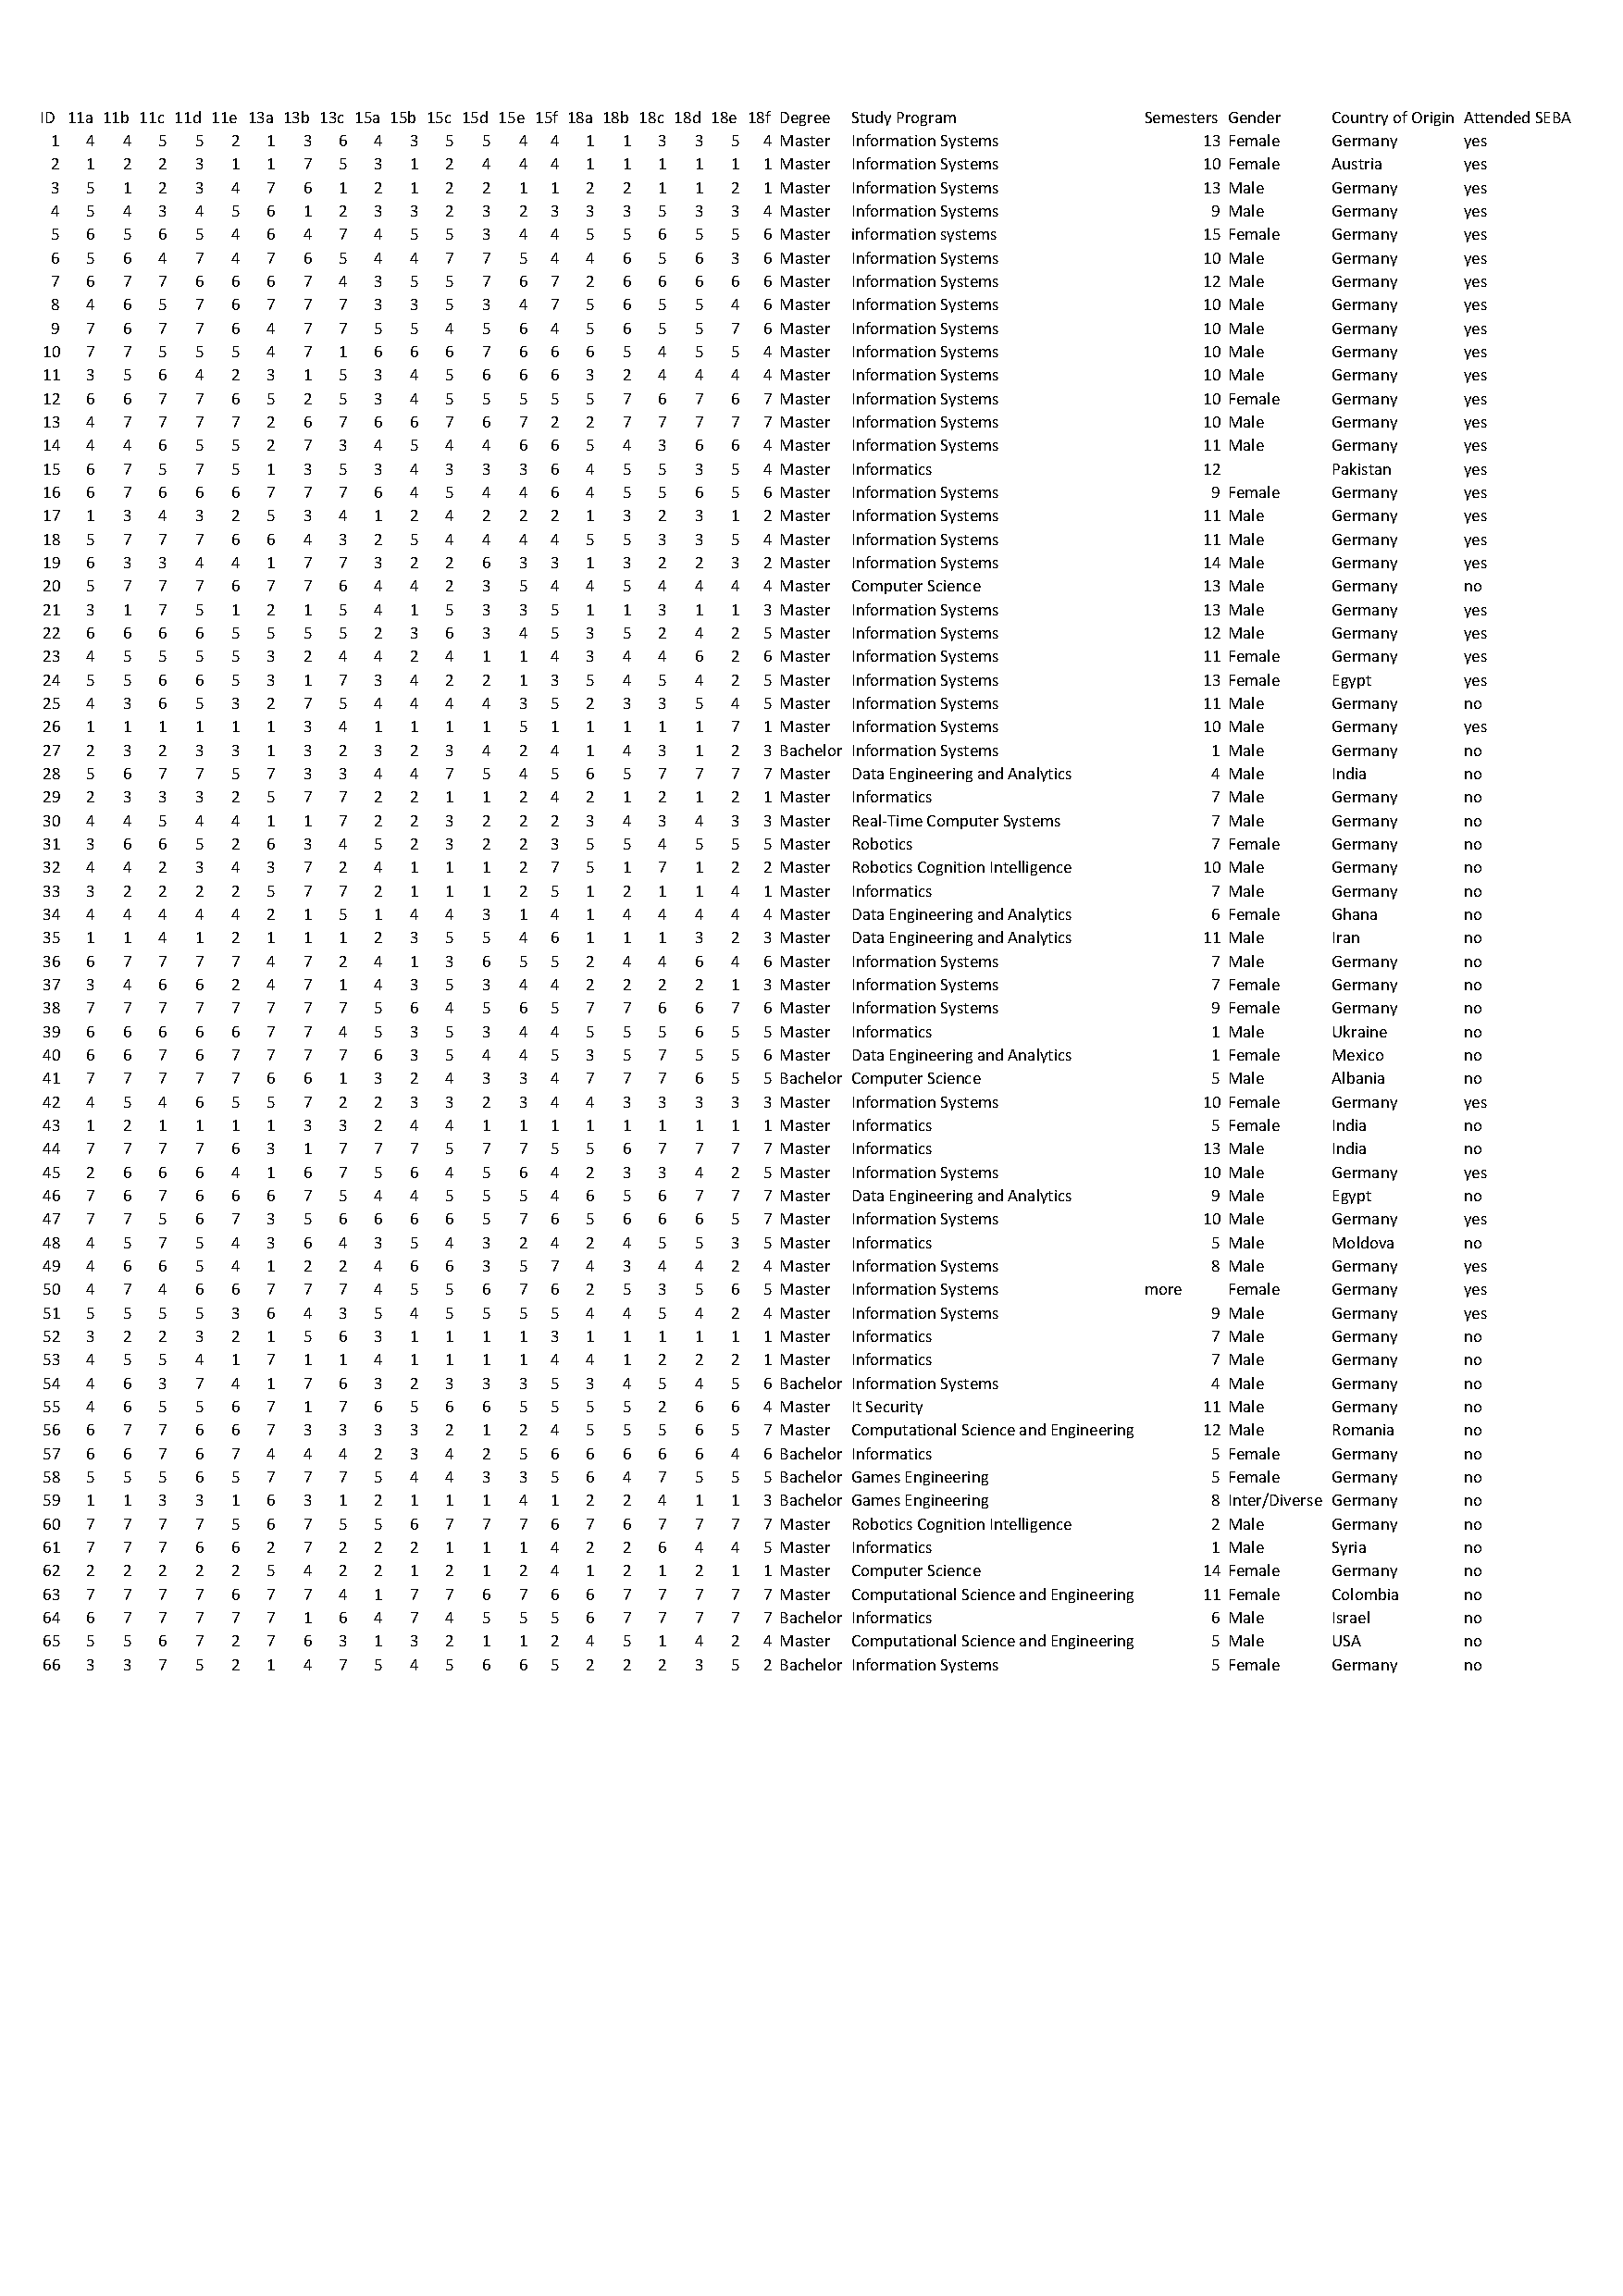
\includegraphics[width=0.98\textwidth]{images/cleaned-responses.pdf}} %factor required, so that latex does not add a blank page 
\end{figure}

\section{Pedagogical Methods}\label{app:gravan}
\begin{figure}[H]
\label{fig:gravan}
\centering{
\caption{Pedagogical methods adapted from \citet{garavan1994entrepreneurship} and \citet{randolph1979designing}}
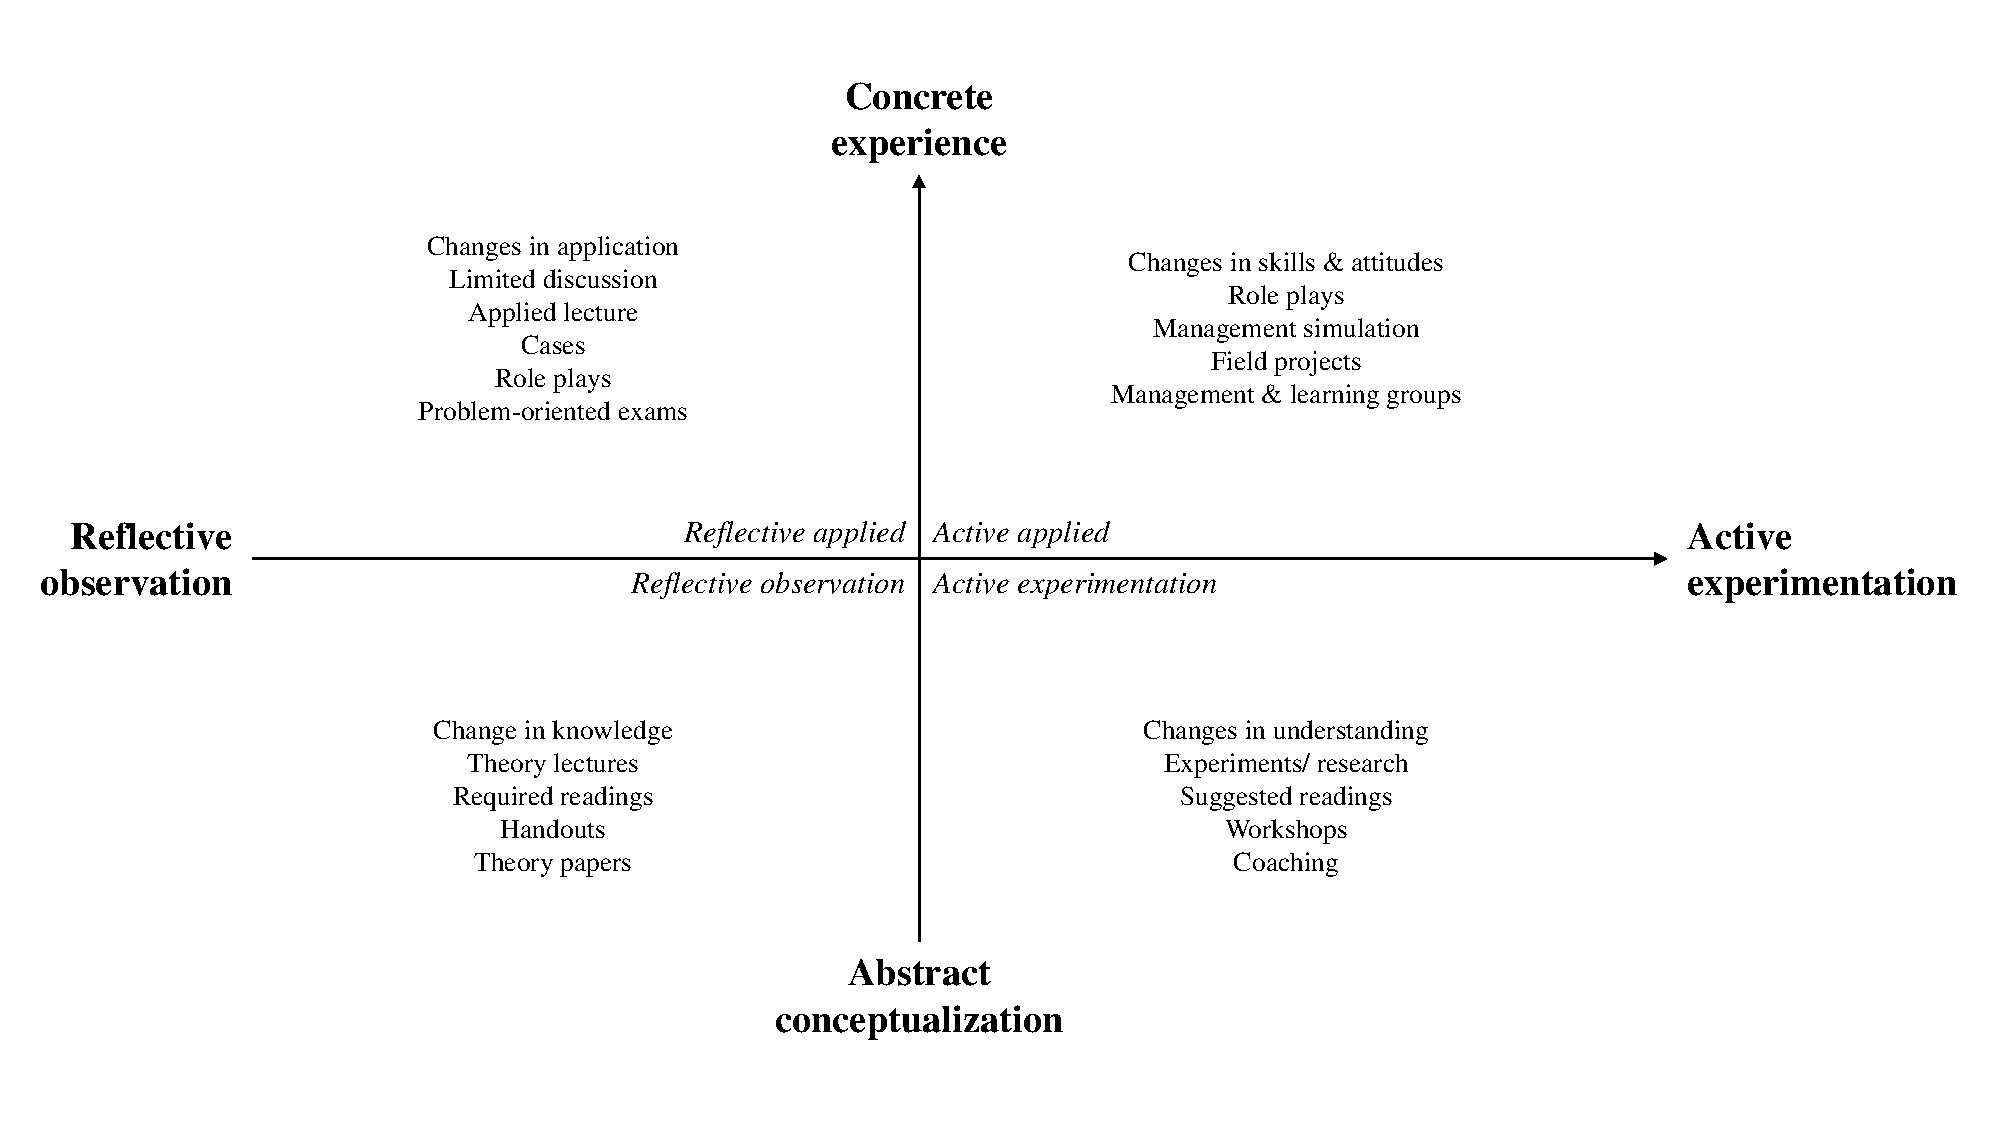
\includegraphics[width=\textwidth]{images/gravan.pdf}}
\end{figure}


\clearpage
\section{Regression Analysis Implementation}\label{section:Appendix Three}
\begin{lstlisting}[basicstyle=\small]
library(dplyr)
library(car)


########   SETTINGS    #############
setwd("/Users/lukasmohs/Desktop/Innovation-Analysis/") 
#adjust to directiory
data = read.csv("cleaned-responses.csv",sep=';')
summary(data)
data <- mutate(
	data, ATB = (X11a+X11b+X11c+X11d+X11e)/5
)
data <- mutate(
	data, SN = (X13a+X13b+X13c)/3
)
data <- mutate(
	data, PBC = (X15a + X15b + X15c + X15d + X15e + X15f)/6
)
data <- mutate(
	data, EI = (X18a + X18b + X18c + X18d + X18e + X18f)/6
)
data <- mutate(
	data, SEBA = ifelse(
    	Attended.SEBA == 'yes', 1, 0
	)
)
data <- mutate(
	data, Entrepreneur = ifelse(
    	Already.Entrepreneur == 'yes', 1, 0
	)
)

########    EFFECT OF EI on ACTION    #############
#Modeling effect of IE on Entrepreneur
fitIEonEntrpreneur <- lm(Entrepreneur ~ EI, data=data)
summary(fitIEonEntrpreneur)

########    EFFECT OF SEBA    #############
#Modeling effect of SEBA on IE
fitSEBAonEI <- lm(EI ~ SEBA, data=data)
summary(fitSEBAonEI)
plot(data$SEBA, data$EI, axes=FALSE, main="SEBA vs. EI", 
     xlab="SEBA ", ylab="EI", pch=19)
axis(side=1, at=c(0:1))
axis(side=2, at=c(1:7))
abline(fitSEBAonEI, col="red")

#Modeling effect of SEBA on ATB
fitATB <- lm(ATB ~ SEBA, data=data)
summary(fitATB)
plot(data$SEBA, data$ATB, axes=FALSE, main="SEBA vs. ATB", 
     xlab="SEBA ", ylab="ATB", pch=19)
axis(side=1, at=c(0:1))
axis(side=2, at=c(1:7))
abline(fitATB, col="red")

#Modeling effect of SEBA on SN
fitSN <- lm(SN ~ SEBA, data=data)
summary(fitSN)
plot(data$SEBA, data$SN, axes=FALSE, main="SEBA vs. SN", 
     xlab="SEBA ", ylab="SN", pch=19)
axis(side=1, at=c(0:1))
axis(side=2, at=c(1:7))
abline(fitSN, col="red")

#Modeling effect of SEBA on PBC
fitPBC <- lm(PBC ~ SEBA, data=data)
summary(fitPBC)
plot(data$SEBA, data$PBC, axes=FALSE, main="SEBA vs. PBC", 
     xlab="SEBA ", ylab="PBC", pch=19)
axis(side=1, at=c(0:1))
axis(side=2, at=c(1:7))
abline(fitPBC, col="red")


########    EFFECT OF AJZEN ANTECEDENT    #############
#Modeling effect of Ajzens antecedents on IE
fitAjzen <- lm(EI ~ ATB + SN + PBC, data=data)
summary(fitAjzen)
#plot(fitAjzen)

#Plot effect of ATB on EI
plot(data$ATB,data$EI,  main="EI vs. ATB", 
     xlab="ATB ", ylab="EI", pch=19)
abline(lm(EI ~ ATB, data = data), col="red")

#Plot effect of SN on EI
plot(data$SN,data$EI,  main="EI vs. SN", 
     xlab="SN ", ylab="EI", pch=19)
abline(lm(EI ~ SN, data = data), col="red")

#Plot effect of PBC on EI
plot(data$PBC,data$EI,  main="EI vs. PBC",
     xlab="PBC ", ylab="EI", pch=19)
abline(lm(EI ~ PBC, data = data), col="red")

\end{lstlisting}
